\documentclass[addpoints]{exam}
\usepackage[utf8x]{inputenc}
\usepackage[ngerman]{babel}
\usepackage{listings}
\usepackage{babel}
\usepackage[top=1.5cm,bottom=0.5cm,headsep=0.5cm,headheight=3cm,%
left=1.5cm,right=1.5cm]{geometry}

\usepackage[T1]{fontenc}
\usepackage{booktabs} % schöne Tabellen
\usepackage{graphicx}
\usepackage{csquotes} % Anführungszeichen
\usepackage{paralist} % kompakte Aufzählungen
\usepackage{amsmath,textcomp,tikz} %diverses
\usepackage{eso-pic} % Bilder im Hintergrund
\usepackage{mdframed} % Boxen
\usepackage{multirow}


\newmdenv[linecolor=black,backgroundcolor=gray!15,
frametitle={Punktverteilung},leftmargin=1cm,
rightmargin=1cm]{infobox}

\lstset{language=Python, tabsize=4, basicstyle=\footnotesize, showstringspaces=false, mathescape=true}
\lstset{literate=%
  {Ö}{{\"O}}1
  {Ä}{{\"A}}1
  {Ü}{{\"U}}1
  {ß}{{\ss}}1
  {ü}{{\"u}}1
  {ä}{{\"a}}1
  {ö}{{\"o}}1
}
\begin{document}
\pointpoints{Punkt}{Punkte}
\bonuspointpoints{Bonuspunkt}{Bonuspunkte}
\renewcommand{\solutiontitle}{\noindent\textbf{Lösung:}%
\enspace}

\chqword{Frage}
\chpgword{Seite}
\chpword{Punkte}
\chbpword{Bonus Punkte}
\chsword{Erreicht}
\chtword{Gesamt}
\hpword{Punkte:} % Punktetabelle
\hsword{Ergebnis:}
\hqword{Aufgabe:}
\htword{Summe:}
\cellwidth{1.5em}
%\begin{center}
%\fbox{\fbox{\parbox{5.5in}{\centering
%Informatik-Klausur}}}
%\end{center}
%
%\vspace{5mm}
%
%\makebox[\textwidth]{Name:\enspace\hrulefill}
\pagestyle{headandfoot}
\runningheadrule

\newcommand\Vtextvisiblespace[1][.3em]{%
  \mbox{\kern.06em\vrule height.3ex}%
  \vbox{\hrule width#1}%
  \hbox{\vrule height.3ex}}

\newcommand{\klaubez}{Aufgaben zu binären Bäumen}
\firstpageheader{Informatik }{\klaubez} {\thepage /\numpages}
\runningheader{Informatik }{\klaubez} {\thepage /\numpages}
\newcommand{\pfad}{c:/MyData/07_Kurse/Kursaufgaben}
%-------------------------------------------------------------------
\printanswers
%-------------------------------------------------------------------

\begin{questions}
\question[4]
a. Zeichne den Baum. \\
b. Traversiere den Baum in inorder, preorder und postorder.
\begin{lstlisting}
...14
..10
...12
.6
...23
..9
1
..7
...13
.14
...12
..3
...11
\end{lstlisting}

\begin{solutionbox}{8cm}
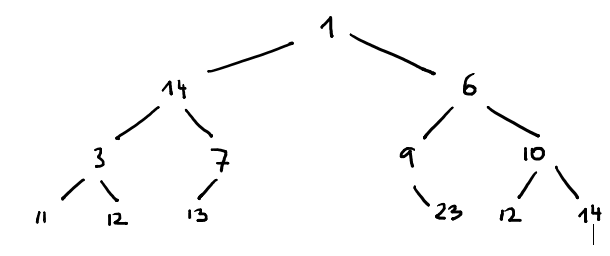
\includegraphics[height=3cm]{\pfad/Baum/Aufgaben/traverse_01/traverse_01.png}
\begin{lstlisting}
inorder: 11 3 12 14 13 7 1 9 23 6 12 10 14
preorder: 1 14 3 11 12 7 13 6 9 23 10 12 14
postorder: 11 12 3 13 7 14 23 9 12 14 10 6 1
\end{lstlisting}
\end{solutionbox}

\question[3]
Schreibe eine Funktion \texttt{baum}, die den abgebildeten Baum zurückgibt.
Nutze dazu unsere Baum-Klasse.
Verschachtele die Baum-Aufrufe aus Lesbarkeitsgründen
höchstens einmal und gib den temporären Teilbäumen sprechende Namen.

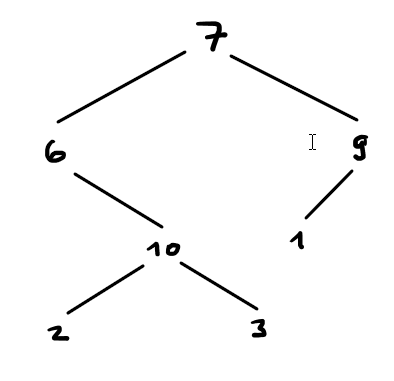
\includegraphics[height=4cm]{\pfad/Baum/Aufgaben/baumdef_01/baumdef_01.png}

\begin{solutionbox}{5cm}
\begin{lstlisting}
def baum():
    b10 = Baum(10,Baum(2),Baum(3))
    b6 = Baum(6,None,b10)
    b9 = Baum(9,Baum(1),None)
    b7 = Baum(7,b6,b9)
    return b7
\end{lstlisting}
\end{solutionbox}



% -------------------------------------------------
\end{questions}
\begin{center}
%\pointtable[h][questions]
\end{center}

\end{document}
